% CaelumFusion VGA View-Selection System - paper extension
%
% Source-aligned final draft section for the Basys-3 VGA renderer.  This file
% is intentionally standalone so it can be compiled for review or copied into a
% larger report/manuscript.

\documentclass{article}

\usepackage[margin=0.75in]{geometry}
\usepackage{amsmath}
\usepackage{amssymb}
\usepackage{array}
\usepackage{booktabs}
\usepackage{longtable}
\usepackage{tabularx}
\usepackage{enumitem}
\usepackage{xcolor}
\usepackage{graphicx}
\usepackage{tikz}
\usetikzlibrary{arrows.meta,positioning,calc,fit}
\usepackage[hidelinks]{hyperref}

\setlength{\parindent}{0pt}
\setlength{\parskip}{5pt}
\renewcommand{\arraystretch}{1.16}
\setlist[itemize]{leftmargin=1.35em,itemsep=2pt,topsep=3pt}
\setlist[enumerate]{leftmargin=1.55em,itemsep=2pt,topsep=3pt}
\emergencystretch=2em

\urlstyle{same}
\newcommand{\sig}[1]{\begingroup\nolinkurl{#1}\endgroup}
\newcommand{\file}[1]{\begingroup\nolinkurl{#1}\endgroup}
\newcommand{\param}[1]{\begingroup\nolinkurl{#1}\endgroup}
\newcommand{\view}[1]{\textsc{#1}}

\definecolor{safegreen}{HTML}{138A36}
\definecolor{warnamber}{HTML}{C77700}
\definecolor{faultred}{HTML}{B42020}
\definecolor{panelblue}{HTML}{1D5F8A}
\definecolor{mutedgray}{HTML}{666666}

\title{\textbf{CaelumFusion VGA View-Selection System}\\Final Engineering Paper Extension}
\author{CaelumFusion Flight Control Project}
\date{July 5, 2026}

\begin{document}
\maketitle

\begin{abstract}
This extension documents the VGA view-selection system used by the
CaelumFusion Basys-3 flight-visualization path.  The section is source-aligned
to the active \file{caelumfusion_top_vga.v},
\file{caelumfusion_vga_render_control.v}, \file{flight_visualizer_pix.v},
\file{flight_vga_page_mux_pix.v}, \file{planar_compass_truth_page_vga.v}, and
\file{Basys-3-Master.xdc} implementation.  The design exposes a small
deterministic view selector, separates registered view navigation from
level-style diagnostic holds, preserves frame-stable telemetry commits, and
drives only the Basys-3 analog VGA interface:
\sig{vga_hsync}, \sig{vga_vsync}, and \sig{vga_rgb[11:0]}.
\end{abstract}

\section{Engineering Intent and Scope}

The VGA view-selection system is an engineering instrument, not a decorative
display mode selector.  Its purpose is to make different classes of evidence
visible on the same 640 by 480 RGB444 VGA output while preserving deterministic
timing, bounded control behavior, and clear truth/representation boundaries.
The active design uses a single board-facing VGA stream and routes selected
rendered content into that stream through two controlled stages:

\begin{enumerate}
  \item the HUD-stream page selector inside \file{flight_visualizer_pix.v},
        which selects the primary flight HUD or the optional sensor diagnostic
        page; and
  \item the optional compass truth-page replacement stage, which can replace
        the already-formed HUD-stream RGB while passing through the same VGA
        sync signals.
\end{enumerate}

The top-level view-control boundary is \file{caelumfusion_vga_render_control.v}.
It accepts SYS-clock view-selection controls that have already been synchronized
and debounced by \file{caelumfusion_top_vga.v}.  The view-control module then
produces independent renderer controls:
\sig{flight_selftest_en_sys}, \sig{vga_page_select_sys}, and
\sig{compass_page_enable_sys}.  This split is essential because self-test data
substitution, HUD-page selection, and full-screen compass replacement are
different engineering states.

\section{Available Display Views}

The registered selector contains four named views.  The compass view is legal
only when \param{USE_COMPASS_TRUTH_PAGE} is nonzero; the sensor diagnostic view
is always a legal selector state, but its diagnostic RGB is present only when
\param{USE_SENSOR_DIAG_PAGE} is nonzero.

\begin{longtable}{p{0.16\linewidth} p{0.20\linewidth} p{0.26\linewidth} p{0.28\linewidth}}
\toprule
\textbf{ID} & \textbf{View name} & \textbf{Renderer path} & \textbf{Engineering use} \\
\midrule
\endhead
\sig{3'd0} &
\sig{VIEW_FLIGHT_HUD} &
Primary \file{flight_visualizer_pix.v} HUD page with live telemetry. &
Default flight-facing engineering display for raw health, derived state,
authority evidence, navigation/wind evidence, and power/I2C diagnostics. \\

\sig{3'd1} &
\sig{VIEW_COMPASS_TRUTH} &
\file{planar_compass_truth_page_vga.v} replaces HUD-stream RGB after the HUD
renderer. &
Full-screen magnetometer/heading diagnostic for planar compass truth,
redundant MAG evidence, sequence alignment, and I2C error evidence. \\

\sig{3'd2} &
\sig{VIEW_SELFTEST_HUD} &
Primary HUD page fed by deterministic self-test substitutions inside
\file{flight_viz_suite_top.v}. &
Renderer bring-up mode.  It verifies layout, history rings, color rules, text,
and visible liveness without requiring live sensors. \\

\sig{3'd3} &
\sig{VIEW_SENSOR_DIAG} &
HUD-stream page select \sig{vga_page_select_sys=2'd1}; final selection occurs
in \file{flight_vga_page_mux_pix.v}. &
Sensor/extension/navigation diagnostic page.  It shows a status matrix,
extension scale bars, and navigation/wind trails when compiled in. \\
\bottomrule
\end{longtable}

\section{Inputs Controlling View Selection}

View selection is driven by three classes of control input.

\begin{itemize}
  \item \textbf{Momentary navigation buttons:} BTNU and BTND create debounced
        one-cycle SYS-domain pulses for next/previous view traversal.
  \item \textbf{Direct request input:} BTNR creates a debounced direct request.
        In the current encoded-selector RTL, SW13:SW11 provide the requested
        view ID only while SW3 MAG1 bench mode and SW2+SW6 diagnostic fault
        injection are inactive.  During either ownership mode the board top
        emits reserved \sig{3'b111}, which is rejected and latched as invalid.
  \item \textbf{Level-style holds and configuration controls:} SW2 can hold the
        self-test HUD, SW4 and SW14 can hold the compass/MAG page, SW5 freezes
        HUD history rings, and wrapper-level control-register style inputs
        provide direct view ID, invalid-view clear, reset view, and page-enable
        policy.
\end{itemize}

\begin{longtable}{p{0.14\linewidth} p{0.24\linewidth} p{0.16\linewidth} p{0.36\linewidth}}
\toprule
\textbf{Board/control} & \textbf{RTL signal} & \textbf{Pin or source} & \textbf{View-selection behavior} \\
\midrule
\endhead
BTNU &
\sig{btn_page_raw} to \sig{view_next_pulse_sys} &
\sig{T18} &
Debounced rising edge advances the registered selected view. \\

BTND &
\sig{btn_prev_raw} to \sig{view_prev_pulse_sys} &
\sig{U17} &
Debounced rising edge moves the registered selected view backward. \\

BTNR &
\sig{btn_direct_compass_raw} to \sig{view_direct_valid_sys},
\sig{view_direct_id_sys[2:0]} &
\sig{T17} &
Loads the encoded SW13:SW11 direct-view ID when SW3 MAG1 bench mode and SW2+SW6
diagnostic fault injection are inactive.  During either SW11--SW13 ownership
mode, the request is forced to reserved \sig{3'b111}; the current view is held
and \sig{cfg_invalid_view_sys} latches. \\

SW3, SW6, SW11--SW13 &
board-level selector ownership inputs &
\sig{W17}, \sig{W14}, \sig{R3/W2/U1} &
SW3 gives SW11--SW13 to MAG1 bench offsets.  SW2+SW6 gives SW11--SW13 to
diagnostic fault-class selection.  Encoded BTNR navigation is blocked during
either ownership mode. \\

SW2 &
\sig{sw_selftest_raw} to \sig{legacy_selftest_hold_sys} &
\sig{W16} &
Holds \sig{VIEW_SELFTEST_HUD} unless compass hold is active.  In the current
top, SW2 is masked out of self-test hold when SW6 log/fault-injection mode is
also active. \\

SW4 &
\sig{sw_compass_page_raw} to \sig{legacy_compass_page_hold_sys} &
\sig{W15} &
Holds \sig{VIEW_COMPASS_TRUTH} when the compass page is compiled in. \\

SW5 &
\sig{sw_history_freeze_raw} to \sig{history_freeze_sys} &
\sig{V15} &
Freezes HUD history-ring updates.  It does not change the selected view. \\

SW14 &
\sig{sw_compass_default_raw} ORed into \sig{legacy_compass_page_hold_sys} &
\sig{T1} &
Runtime companion hold for the compass/MAG evidence page. \\

Wrapper direct ID &
\sig{view_direct_valid_sys}, \sig{view_direct_id_sys[2:0]} &
control-register style interface &
Requests an exact view ID.  Legal IDs are accepted; illegal IDs latch
\sig{cfg_invalid_view_sys} and leave \sig{view_sel_sys} unchanged. \\

Wrapper clear &
\sig{cfg_invalid_view_clear_sys} &
control-register style interface &
Clears the invalid-view latch inside the wrapper.  The active board top ties
this input low, so the board-level clear mechanism is reset-only. \\
\bottomrule
\end{longtable}

\section{Navigation and Priority Rules}

The registered view state \sig{view_sel_sys} changes only on legal direct,
next, or previous requests.  The effective view \sig{view_effective_sys} is
then formed by applying level-style holds.  The resulting priority is:

\begin{enumerate}
  \item \textbf{Compass-page hold:} if \sig{legacy_compass_page_hold_sys=1} and
        \param{USE_COMPASS_TRUTH_PAGE != 0}, the effective view is
        \sig{VIEW_COMPASS_TRUTH}.
  \item \textbf{Self-test hold:} if compass hold is not active and
        \sig{legacy_selftest_hold_sys=1}, the effective view is
        \sig{VIEW_SELFTEST_HUD}.
  \item \textbf{Registered view:} otherwise, the effective view is
        \sig{view_sel_sys}.
\end{enumerate}

The normal next sequence is:
\begin{center}
\sig{VIEW_FLIGHT_HUD}
\(\rightarrow\) \sig{VIEW_SENSOR_DIAG}
\(\rightarrow\) \sig{VIEW_COMPASS_TRUTH}
\(\rightarrow\) \sig{VIEW_SELFTEST_HUD}
\(\rightarrow\) \sig{VIEW_FLIGHT_HUD}.
\end{center}
When \param{USE_COMPASS_TRUTH_PAGE=0}, the next/previous functions skip
\sig{VIEW_COMPASS_TRUTH}.  They do not skip \sig{VIEW_SENSOR_DIAG}; if
\param{USE_SENSOR_DIAG_PAGE=0}, that registered view falls back visually to
the primary HUD stream.

\begin{figure}[htbp]
\centering
\resizebox{0.94\linewidth}{!}{%
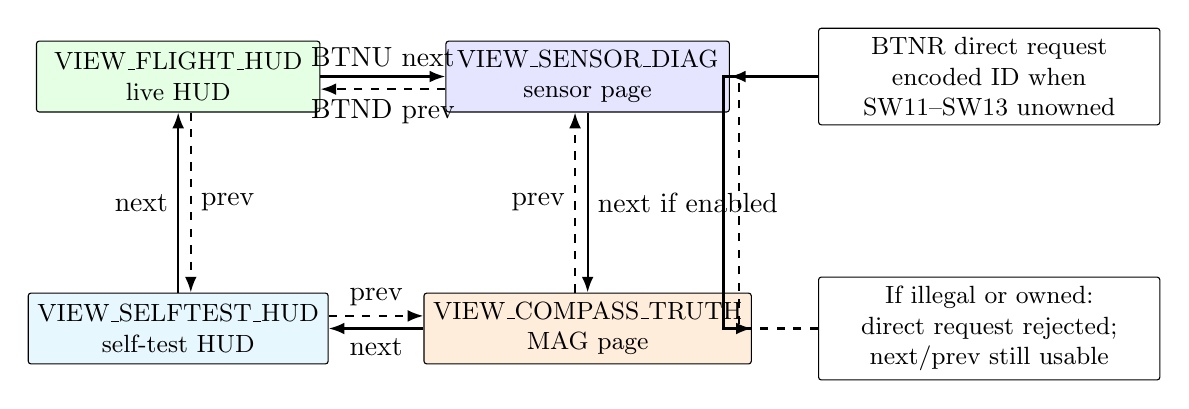
\begin{tikzpicture}[
  state/.style={draw, rounded corners=1pt, minimum width=3.6cm, minimum height=0.9cm, align=center, font=\small},
  arr/.style={-{Latex[length=2mm]}, thick},
  prev/.style={-{Latex[length=2mm]}, thick, dashed},
  note/.style={draw, rounded corners=1pt, align=center, font=\small, text width=4.1cm}
]
\node[state, fill=green!10] at (0,2.0) (hud) {\sig{VIEW\_FLIGHT\_HUD}\\live HUD};
\node[state, fill=blue!10] at (5.2,2.0) (diag) {\sig{VIEW\_SENSOR\_DIAG}\\sensor page};
\node[state, fill=orange!14] at (5.2,-1.2) (truth) {\sig{VIEW\_COMPASS\_TRUTH}\\MAG page};
\node[state, fill=cyan!10] at (0,-1.2) (self) {\sig{VIEW\_SELFTEST\_HUD}\\self-test HUD};

\draw[arr] (hud.east) -- node[above]{BTNU next} (diag.west);
\draw[arr] (diag.south) -- node[right]{next if enabled} (truth.north);
\draw[arr] (truth.west) -- node[below]{next} (self.east);
\draw[arr] (self.north) -- node[left]{next} (hud.south);

\draw[prev] ([yshift=-0.16cm]diag.west) -- node[below]{BTND prev} ([yshift=-0.16cm]hud.east);
\draw[prev] ([xshift=-0.16cm]truth.north) -- node[left]{prev} ([xshift=-0.16cm]diag.south);
\draw[prev] ([yshift=0.16cm]self.east) -- node[above]{prev} ([yshift=0.16cm]truth.west);
\draw[prev] ([xshift=0.16cm]hud.south) -- node[right]{prev} ([xshift=0.16cm]self.north);

\node[note] at (10.3,2.0) (direct) {BTNR direct request\\encoded ID when\\SW11--SW13 unowned};
\node[note] at (10.3,-1.2) (fallback) {If illegal or owned:\\direct request rejected;\\next/prev still usable};
\draw[arr] (direct.west) -- ++(-1.2,0) |- (truth.east);
\draw[prev] (fallback.west) -- ++(-1.0,0) |- (diag.east);
\end{tikzpicture}}
\caption{VGA view-selection navigation.  Solid paths are next/direct requests;
dashed paths are previous or disabled-feature behavior.}
\label{fig:vga-view-navigation}
\end{figure}

\section{Control-to-Renderer Mapping}

Figure~\ref{fig:control-renderer-map-final} shows the complete control path
from human inputs and control-register style fields to final VGA output.  All
button and switch inputs are asynchronous at the package pin and are first
synchronized in the board top.  Only debounced pulses or stable levels enter
\file{caelumfusion_vga_render_control.v}.

\begin{figure}[htbp]
\centering
\resizebox{\linewidth}{!}{%
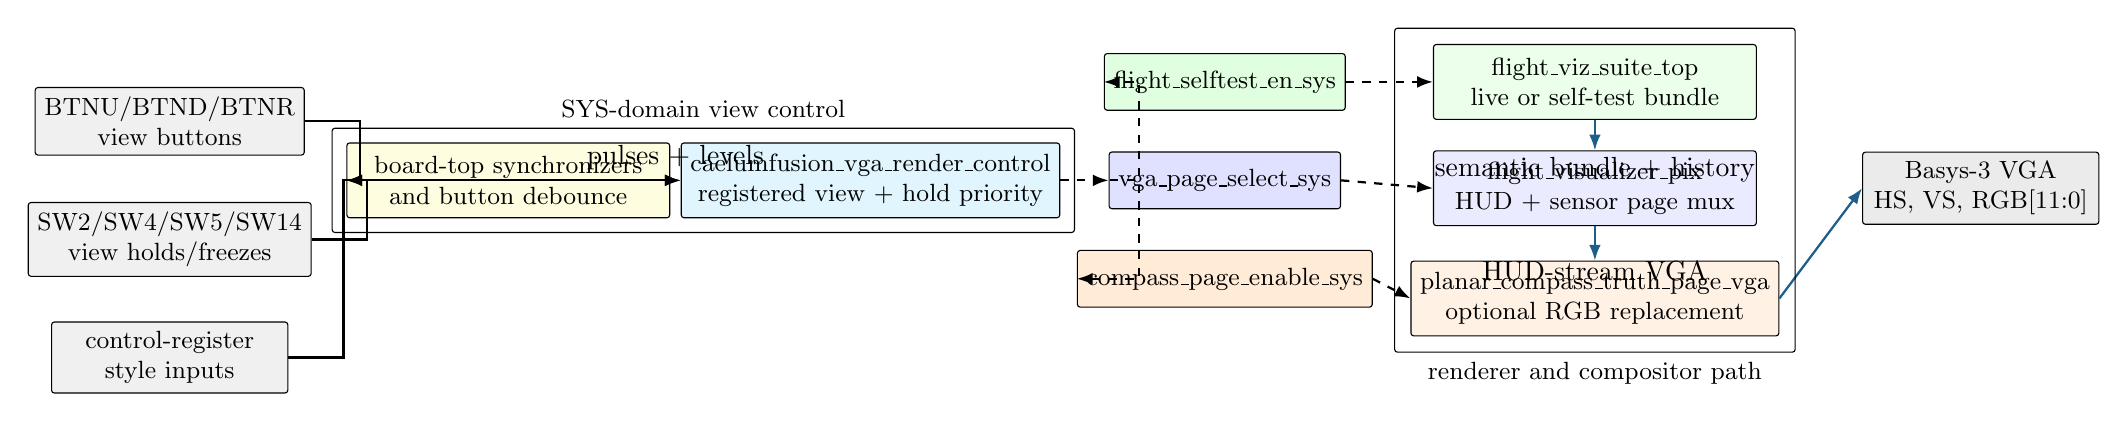
\begin{tikzpicture}[
  box/.style={draw, rounded corners=1pt, minimum width=3.0cm, minimum height=0.82cm, align=center, font=\small},
  wide/.style={draw, rounded corners=1pt, minimum width=4.1cm, minimum height=0.95cm, align=center, font=\small},
  smallbox/.style={draw, rounded corners=1pt, minimum width=2.8cm, minimum height=0.72cm, align=center, font=\small},
  arr/.style={-{Latex[length=2mm]}, thick},
  ctrl/.style={-{Latex[length=2mm]}, thick, dashed},
  bus/.style={-{Latex[length=2mm]}, thick, draw=panelblue}
]
\node[box, fill=gray!12] at (0,3.0) (buttons) {BTNU/BTND/BTNR\\view buttons};
\node[box, fill=gray!12] at (0,1.5) (switches) {SW2/SW4/SW5/SW14\\view holds/freezes};
\node[box, fill=gray!12] at (0,0.0) (regs) {control-register\\style inputs};

\node[wide, fill=yellow!12] at (4.3,2.25) (sync) {board-top synchronizers\\and button debounce};
\node[wide, fill=cyan!12] at (8.9,2.25) (logic) {\file{caelumfusion\_vga\_render\_control}\\registered view + hold priority};

\node[smallbox, fill=green!12] at (13.4,3.5) (selfctl) {\sig{flight\_selftest\_en\_sys}};
\node[smallbox, fill=blue!12] at (13.4,2.25) (pagectl) {\sig{vga\_page\_select\_sys}};
\node[smallbox, fill=orange!16] at (13.4,1.0) (compctl) {\sig{compass\_page\_enable\_sys}};

\node[wide, fill=green!8] at (18.1,3.5) (suite) {\file{flight\_viz\_suite\_top}\\live or self-test bundle};
\node[wide, fill=blue!8] at (18.1,2.15) (pix) {\file{flight\_visualizer\_pix}\\HUD + sensor page mux};
\node[wide, fill=orange!10] at (18.1,0.75) (truth) {\file{planar\_compass\_truth\_page\_vga}\\optional RGB replacement};
\node[box, fill=black!8] at (23.0,2.15) (vga) {Basys-3 VGA\\\sig{HS}, \sig{VS}, \sig{RGB[11:0]}};

\draw[arr] (buttons.east) -- ++(0.7,0) |- (sync.west);
\draw[arr] (switches.east) -- ++(0.7,0) |- (sync.west);
\draw[arr] (regs.east) -- ++(0.7,0) |- (logic.west);
\draw[ctrl] (sync.east) -- node[above]{pulses + levels} (logic.west);

\draw[ctrl] (logic.east) -- ++(1.0,0) |- (selfctl.west);
\draw[ctrl] (logic.east) -- (pagectl.west);
\draw[ctrl] (logic.east) -- ++(1.0,0) |- (compctl.west);

\draw[ctrl] (selfctl.east) -- (suite.west);
\draw[bus] (suite.south) -- ++(0,-0.35) -| node[pos=0.25,below]{semantic bundle + history} (pix.north);
\draw[ctrl] (pagectl.east) -- (pix.west);
\draw[bus] (pix.south) -- ++(0,-0.32) -| node[pos=0.25,below]{HUD-stream VGA} (truth.north);
\draw[ctrl] (compctl.east) -- (truth.west);
\draw[bus] (truth.east) -- (vga.west);

\node[draw, rounded corners=1pt, fit=(sync) (logic), inner sep=0.18cm, label={[font=\small]above:SYS-domain view control}] {};
\node[draw, rounded corners=1pt, fit=(suite) (pix) (truth), inner sep=0.20cm, label={[font=\small]below:renderer and compositor path}] {};
\end{tikzpicture}}
\caption{Control-to-renderer mapping for VGA view selection.  Dashed arrows are
control enables; blue solid arrows are rendered telemetry or VGA streams.}
\label{fig:control-renderer-map-final}
\end{figure}

\section{View Layout and Viewport Locations}

The renderer uses fixed layouts.  This is deliberate: the display remains
scannable during faults because widgets degrade by color, hatching, or marker
suppression rather than by reflowing.

\begin{longtable}{p{0.24\linewidth} p{0.18\linewidth} p{0.48\linewidth}}
\toprule
\textbf{Region} & \textbf{Coordinates} & \textbf{Owned content} \\
\midrule
\endhead
Top strip & \sig{y=0..27} & BMP, ACC, and MAG raw validity/status/age/sequence health. \\
Text/title band & \sig{y=28..105} & Fixed panel titles and telemetry rows. \\
Column 0 & \sig{x=0..212}, \sig{y=106..359} & Altitude tape, vertical-speed tape, and apogee authority ladder. \\
Column 1 & \sig{x=213..425}, \sig{y=106..359} & Artificial horizon and roll-plane vector. \\
Column 2 & \sig{x=426..639}, \sig{y=106..359} & Compass rose and landing/wind viewport. \\
Altitude chart & \sig{y=360..415} & BRAM-backed altitude history. \\
Vertical-speed chart & \sig{y=416..467} & BRAM-backed vertical-speed history. \\
Bottom debug strip & \sig{y=468..479} & PMON1 and I2C debug evidence. \\
\midrule
Sensor matrix & \sig{x=8..314}, \sig{y=36..284} & BMP, ACC, MAG, PWR, derived, extension, navigation, and wind rows. \\
Extension scales & \sig{x=330..628}, \sig{y=36..222} & Range, air, environment, sun, and flow scale bars. \\
Navigation/wind trail & \sig{x=330..628}, \sig{y=246..452} & Sixteen-sample navigation and wind trace. \\
\bottomrule
\end{longtable}

\begin{figure}[htbp]
\centering
\resizebox{\linewidth}{!}{%
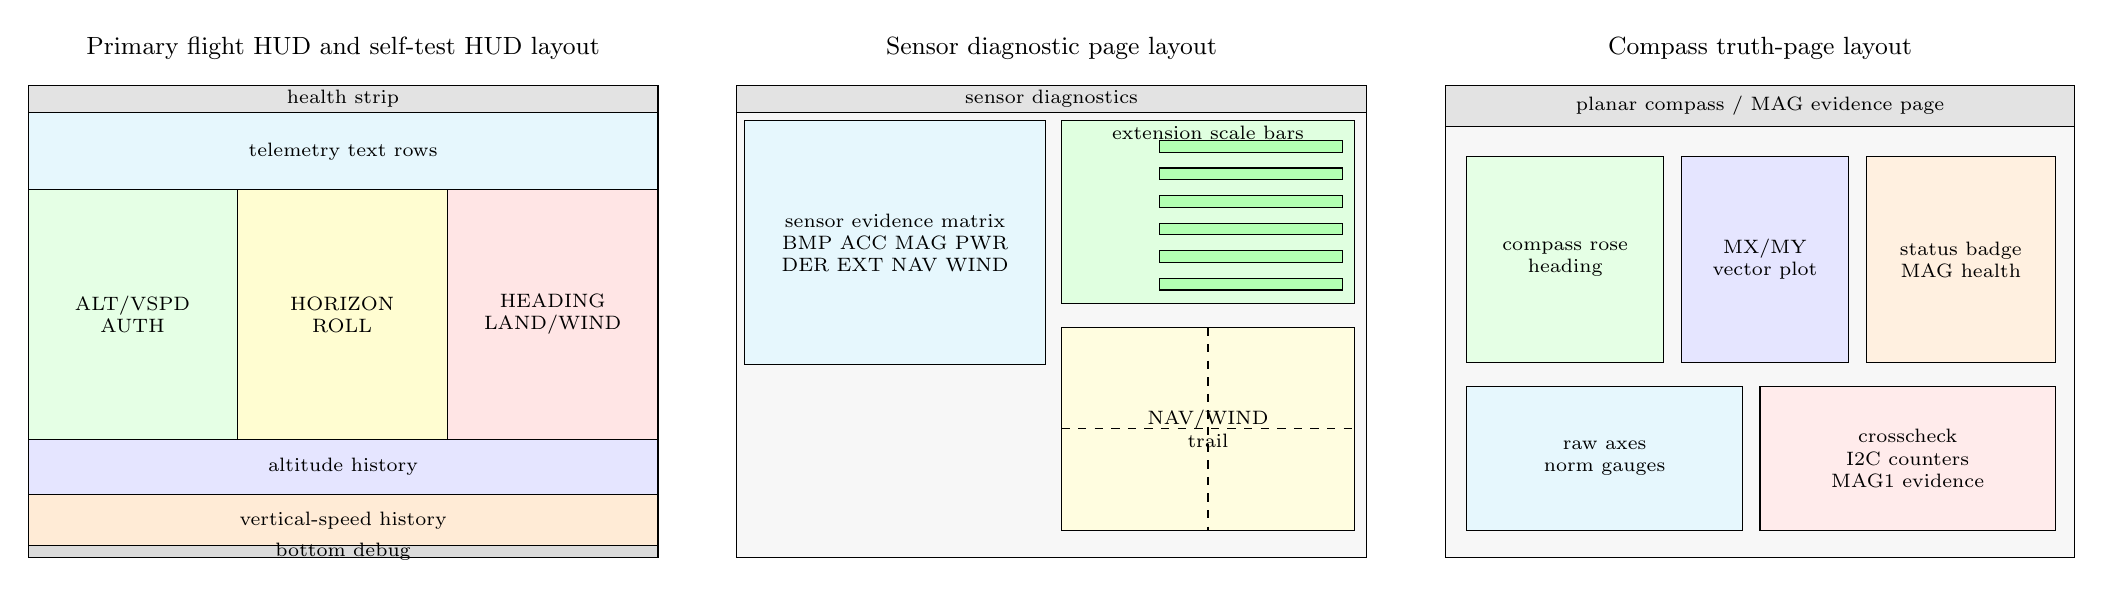
\begin{tikzpicture}[x=0.0125cm,y=-0.0125cm,font=\scriptsize]
  \begin{scope}
    \draw[fill=black!3, draw=black] (0,0) rectangle (640,480);
    \draw[fill=gray!22, draw=black] (0,0) rectangle (640,28);
    \node at (320,14) {health strip};
    \draw[fill=cyan!10, draw=black] (0,28) rectangle (640,106);
    \node at (320,67) {telemetry text rows};
    \draw[fill=green!10, draw=black] (0,106) rectangle (213,360);
    \node[align=center] at (106,233) {ALT/VSPD\\AUTH};
    \draw[fill=yellow!18, draw=black] (213,106) rectangle (426,360);
    \node[align=center] at (319,233) {HORIZON\\ROLL};
    \draw[fill=red!10, draw=black] (426,106) rectangle (640,360);
    \node[align=center] at (533,233) {HEADING\\LAND/WIND};
    \draw[fill=blue!10, draw=black] (0,360) rectangle (640,416);
    \node at (320,388) {altitude history};
    \draw[fill=orange!16, draw=black] (0,416) rectangle (640,468);
    \node at (320,442) {vertical-speed history};
    \draw[fill=gray!28, draw=black] (0,468) rectangle (640,480);
    \node at (320,474) {bottom debug};
    \node[font=\small] at (320,-38) {Primary flight HUD and self-test HUD layout};
  \end{scope}

  \begin{scope}[shift={(720,0)}]
    \draw[fill=black!3, draw=black] (0,0) rectangle (640,480);
    \draw[fill=gray!22, draw=black] (0,0) rectangle (640,28);
    \node at (320,14) {sensor diagnostics};
    \draw[fill=cyan!10, draw=black] (8,36) rectangle (314,284);
    \node[align=center] at (161,160) {sensor evidence matrix\\BMP ACC MAG PWR\\DER EXT NAV WIND};
    \draw[fill=green!12, draw=black] (330,36) rectangle (628,222);
    \node at (479,48) {extension scale bars};
    \foreach \yy in {56,84,112,140,168,196} {
      \draw[fill=green!30, draw=black] (430,\yy) rectangle (616,\yy+12);
    }
    \draw[fill=yellow!12, draw=black] (330,246) rectangle (628,452);
    \draw[dashed] (479,246) -- (479,452);
    \draw[dashed] (330,349) -- (628,349);
    \node[align=center] at (479,349) {NAV/WIND\\trail};
    \node[font=\small] at (320,-38) {Sensor diagnostic page layout};
  \end{scope}

  \begin{scope}[shift={(1440,0)}]
    \draw[fill=black!3, draw=black] (0,0) rectangle (640,480);
    \draw[fill=gray!22, draw=black] (0,0) rectangle (640,42);
    \node at (320,21) {planar compass / MAG evidence page};
    \draw[fill=green!10, draw=black] (22,72) rectangle (222,282);
    \node[align=center] at (122,177) {compass rose\\heading};
    \draw[fill=blue!10, draw=black] (240,72) rectangle (410,282);
    \node[align=center] at (325,177) {MX/MY\\vector plot};
    \draw[fill=orange!12, draw=black] (428,72) rectangle (620,282);
    \node[align=center] at (524,177) {status badge\\MAG health};
    \draw[fill=cyan!10, draw=black] (22,306) rectangle (302,452);
    \node[align=center] at (162,379) {raw axes\\norm gauges};
    \draw[fill=red!8, draw=black] (320,306) rectangle (620,452);
    \node[align=center] at (470,379) {crosscheck\\I2C counters\\MAG1 evidence};
    \node[font=\small] at (320,-38) {Compass truth-page layout};
  \end{scope}
\end{tikzpicture}}
\caption{Screen layout arrangements for the selectable VGA views.}
\label{fig:vga-screen-layouts}
\end{figure}

\section{Compositor Layer Behavior}

The compositor is a priority encoder, not a blending engine.  RGB444 values are
selected deterministically.  Within the primary HUD page, later instrument
conditions intentionally override low-salience grid pixels.  The HUD-stream
page mux then applies active-video blacking and HUD-only text overlay.  Finally,
the optional compass truth page can replace the already-formed HUD-stream RGB.

\begin{figure}[htbp]
\centering
\resizebox{0.86\linewidth}{!}{%
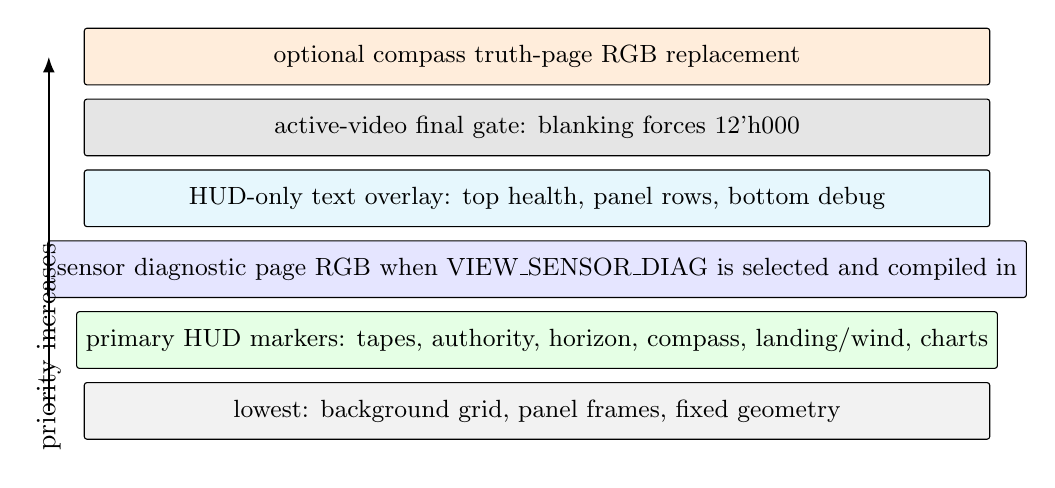
\begin{tikzpicture}[
  layer/.style={draw, rounded corners=1pt, minimum width=11.5cm, minimum height=0.72cm, align=center, font=\small},
  arr/.style={-{Latex[length=2mm]}, thick}
]
\node[layer, fill=gray!10] at (0,0) (grid) {lowest: background grid, panel frames, fixed geometry};
\node[layer, fill=green!10] at (0,0.90) (hud) {primary HUD markers: tapes, authority, horizon, compass, landing/wind, charts};
\node[layer, fill=blue!10] at (0,1.80) (diag) {sensor diagnostic page RGB when \sig{VIEW\_SENSOR\_DIAG} is selected and compiled in};
\node[layer, fill=cyan!10] at (0,2.70) (text) {HUD-only text overlay: top health, panel rows, bottom debug};
\node[layer, fill=black!10] at (0,3.60) (blank) {active-video final gate: blanking forces \sig{12'h000}};
\node[layer, fill=orange!14] at (0,4.50) (truth) {optional compass truth-page RGB replacement};
\draw[arr] (-6.2,0) -- node[left, rotate=90]{priority increases} (-6.2,4.5);
\end{tikzpicture}}
\caption{Compositor layer stack for the VGA stream.}
\label{fig:vga-layer-stack}
\end{figure}

\section{Telemetry Widgets Shown in Each Mode}

\begin{longtable}{p{0.19\linewidth} p{0.34\linewidth} p{0.37\linewidth}}
\toprule
\textbf{Mode} & \textbf{Visible widgets} & \textbf{Primary debugging usefulness} \\
\midrule
\endhead
\sig{VIEW_FLIGHT_HUD} &
Top BMP/ACC/MAG health strip; derived altitude, vertical speed, roll, and
heading text; altitude and vertical-speed tapes; apogee authority ladder;
artificial horizon; roll vector; compass rose; landing/wind viewport; altitude
and vertical-speed charts; bottom PMON/I2C strip. &
Normal integrated telemetry review.  Best for checking whether raw evidence,
derived estimates, authority policy, and display representation agree during
bench operation. \\

\sig{VIEW_SELFTEST_HUD} &
Same HUD geometry as \sig{VIEW_FLIGHT_HUD}, but source fields are deterministic
self-test substitutions for raw summaries, derived state, navigation/wind,
authority, power, counters, build ID, and schema. &
Renderer and cable bring-up.  A visible, stable HUD in this mode proves the
pixel renderer, text compositor, history graphics, and color paths without
depending on live sensor transactions. \\

\sig{VIEW_SENSOR_DIAG} &
Sensor evidence matrix; extension scale bars for range, airspeed, temperature,
humidity, sun/luma, and optical flow; navigation/wind trail viewport.  Normal
HUD text overlay is suppressed. &
Sensor and extension triage.  Best for seeing which evidence source is invalid,
stale, faulted, or absent without interpreting the full flight HUD. \\

\sig{VIEW_COMPASS_TRUTH} &
Planar heading page; compass rose; raw primary MAG vector; 16-sample trail;
redundant MAG1 vector/evidence; norm gauges; derived-heading crosscheck; I2C
NACK/timeout/transaction-rate fields. &
Magnetometer/heading checkout.  Best for diagnosing planar heading, redundant
MAG alignment, sector disagreement, raw/status faults, and I2C health. \\
\bottomrule
\end{longtable}

\section{Widget Enable and Degradation Controls}

Most widgets are not individually disabled by switches.  The stronger
engineering contract is that layout remains fixed while data quality is encoded
using color, hatching, marker suppression, or history freeze.

\begin{longtable}{p{0.25\linewidth} p{0.28\linewidth} p{0.37\linewidth}}
\toprule
\textbf{Widget or page} & \textbf{Enable/control source} & \textbf{Fallback behavior} \\
\midrule
\endhead
Primary HUD widgets &
Active whenever \sig{VIEW_FLIGHT_HUD} or \sig{VIEW_SELFTEST_HUD} is the
effective view, or when optional pages are disabled. &
Frames stay visible.  Invalid or stale telemetry changes semantic color and
may suppress point markers rather than moving layout. \\

History charts &
Committed altitude and vertical speed samples; SW5
\sig{history_freeze_sys}. &
When frozen, chart memory stops accepting new samples; the current displayed
history remains stable for inspection. \\

Sensor diagnostic page &
\param{USE_SENSOR_DIAG_PAGE} and \sig{VIEW_SENSOR_DIAG}. &
If compiled out, \sig{VIEW_SENSOR_DIAG} remains selectable but emits the
primary HUD page RGB. \\

Compass truth page &
\param{USE_COMPASS_TRUTH_PAGE}; BTNR direct request; SW4/SW14 compass hold;
\sig{COMPASS_TRUTH_PAGE_DEFAULT}. &
If compiled out, direct requests are rejected and held compass requests are
gated off.  If compiled in but inactive, the page passes HUD-stream sync/RGB
through. \\

Self-test HUD stimulus &
SW2, unless SW2 is being used with SW6 for diagnostic fault injection. &
Self-test changes the data source, not the HUD layout.  Compass-page hold has
higher priority and can mask the self-test HUD visually. \\
\bottomrule
\end{longtable}

\section{Color Conventions}

The VGA interface is RGB444.  Colors are semantic and intentionally coarse.
They communicate evidence quality and source identity rather than aesthetic
state.

\begin{longtable}{p{0.18\linewidth} p{0.22\linewidth} p{0.50\linewidth}}
\toprule
\textbf{Color family} & \textbf{Representative RGB444 codes} & \textbf{Meaning} \\
\midrule
\endhead
Black & \sig{12'h000} & Reset/blanking, inactive video, and empty background. \\
Dim gray/grid & \sig{12'h011}, \sig{12'h022}, \sig{12'h044}, \sig{12'h111} & Low-salience frames, grids, and inactive context. \\
White & \sig{12'hFFF}, \sig{12'hCCC}, \sig{12'hAAA} & Labels, reference axes, current markers, and clean non-warning text. \\
Green & \sig{12'h0F4}, \sig{12'h2F6}, \sig{12'h2B5} & Valid, fresh, reachable, aligned, allowed, or otherwise positive evidence. \\
Cyan/blue & \sig{12'h0FF}, \sig{12'h3FF}, \sig{12'h08F} & Heading/vector accents, redundant/reference identity, and instrumentation accents. \\
Yellow/amber & \sig{12'hFF0}, \sig{12'hFD0}, \sig{12'hD93} & Stale, warning, sequence mismatch, freshness miss, or caution state. \\
Orange & \sig{12'hF80}, \sig{12'hF50}, \sig{12'hF42} & Degraded active diagnostic state, command/braking emphasis, or warning fill. \\
Red & \sig{12'hF22}, \sig{12'hF50}, \sig{12'hD33} & Invalid, faulted, denied, unsafe, or disagreeing evidence. \\
Magenta & \sig{12'hF0F} & MAG vector or brake/target emphasis where a distinct accent is needed. \\
\bottomrule
\end{longtable}

\section{Default and Fallback Behavior}

The source-default board parameters compile a HUD-only image:
\begin{center}
\param{USE_COMPASS_TRUTH_PAGE=0}, \quad
\param{USE_SENSOR_DIAG_PAGE=0}, \quad
\param{COMPASS_TRUTH_PAGE_DEFAULT=0}.
\end{center}
Therefore reset selects \sig{VIEW_FLIGHT_HUD} unless a build changes the reset
view policy.  Illegal reset IDs are coerced to a legal view, and invalid direct
view IDs hold the current selection while latching \sig{cfg_invalid_view_sys}.

\begin{longtable}{p{0.28\linewidth} p{0.62\linewidth}}
\toprule
\textbf{Condition} & \textbf{Display behavior} \\
\midrule
\endhead
Power-on/reset & VGA timing and RGB return to deterministic idle/black until
pixel reset releases and a committed bundle is available. \\
Compass page compiled out & BTNR direct compass request or encoded ID
\sig{3'd1} is rejected; SW4/SW14 holds are gated off; final RGB remains the HUD
stream. \\
SW11--SW13 owned by MAG1 bench or fault injection & BTNR encoded direct
selection emits reserved \sig{3'b111}; \sig{view_sel_sys} is held and
\sig{cfg_invalid_view_sys} latches. \\
Sensor diagnostic page compiled out & \sig{VIEW_SENSOR_DIAG} remains a legal
registered state, but the PIX page mux selects the primary HUD page. \\
Inactive video/blanking & \file{flight_vga_page_mux_pix.v} forces
\sig{vga_rgb=12'h000}. \\
Raw or derived evidence invalid & Widgets remain in place and degrade through
semantic color, hatching, or marker suppression. \\
Compass hold and self-test hold both active & Compass/MAG page hold wins when
the compass page is compiled in; otherwise self-test HUD can remain visible. \\
Invalid-view latch set & The wrapper supports a clear input, but the current
board top ties it low; reset is the board-level clear. \\
\bottomrule
\end{longtable}

\section{Known Rendering Limitations}

\begin{itemize}
  \item \textbf{View-state observability is internal.}  The active top-level
        wires \sig{view_sel_sys}, \sig{view_effective_sys}, and
        \sig{cfg_invalid_view_sys} are not yet routed to LEDs, UART, or a HUD
        debug field.
  \item \textbf{Optional pages change resource cost.}  Compass truth and sensor
        diagnostic pages should be synthesized and implemented as explicit
        build variants before timing or LUT margin claims are made.
  \item \textbf{Button debounce is fixed.}  The board top uses a deterministic
        \sig{STABLE_CYCLES=250000} debounce interval.  Very rapid taps inside
        the debounce window are intentionally ignored.
  \item \textbf{Sensor diagnostic selection can look like no change in the
        default build.}  With \param{USE_SENSOR_DIAG_PAGE=0}, the state is legal
        but the visible page is the HUD.
  \item \textbf{RGB precision is RGB444.}  Fine gradients, anti-aliased text,
        and subtle color encodings are intentionally unavailable on the Basys-3
        resistor-DAC VGA path.
  \item \textbf{The VGA clock is 25.000 MHz.}  The generated pixel clock is a
        practical 640 by 480 lab-compatible clock, not the nominal 25.175 MHz
        VGA clock; the resulting frame rate is approximately 59.524 Hz.
\end{itemize}

\section{Recommended Verification and Development Steps}

\begin{enumerate}
  \item Add a focused testbench for \file{caelumfusion_vga_render_control.v}
        covering reset coercion, next/previous traversal, direct-view rejection,
        hold priority, and invalid-view latch clear behavior.
  \item Add pixel-level checks for \param{USE_SENSOR_DIAG_PAGE=0} fallback and
        \param{USE_SENSOR_DIAG_PAGE=1} text-overlay suppression.
  \item Expose \sig{view_effective_sys} and \sig{cfg_invalid_view_sys} on a
        bench-visible channel such as LEDs, UART, or a small HUD field.
  \item Run implementation deltas for the source-default HUD build, a compass
        page build, and a sensor diagnostic page build.
  \item Capture bench evidence for reset default, next/previous navigation,
        encoded direct requests with SW11:SW13 unowned, BTNR rejection during
        MAG1 bench or SW2+SW6 fault-injection ownership, self-test hold,
        history freeze, invalid sensor degradation, and compass truth-page
        operation.
\end{enumerate}

\section{Conclusion}

The CaelumFusion VGA view-selection system is a bounded, deterministic
selection layer over a frame-stable telemetry renderer.  It separates human
navigation, direct diagnostic requests, legacy level holds, self-test data
substitution, HUD-page selection, and final full-screen compass replacement.
The resulting architecture supports normal flight visualization, renderer
self-test, sensor/extension diagnostics, and magnetometer truth inspection
without changing the board-facing VGA contract.  The remaining engineering
work is not architectural selection logic; it is verification closure,
bench-visible view-state observability, and build-specific implementation
evidence for optional diagnostic pages.

\end{document}
